\documentclass[ignorenonframetext,]{beamer}
\setbeamertemplate{caption}[numbered]
\setbeamertemplate{caption label separator}{: }
\setbeamercolor{caption name}{fg=normal text.fg}
\beamertemplatenavigationsymbolsempty
\usepackage{lmodern}
\usepackage{amssymb,amsmath}
\usepackage{ifxetex,ifluatex}
\usepackage{fixltx2e} % provides \textsubscript
\ifnum 0\ifxetex 1\fi\ifluatex 1\fi=0 % if pdftex
\usepackage[T1]{fontenc}
\usepackage[utf8]{inputenc}
\else % if luatex or xelatex
\ifxetex
\usepackage{mathspec}
\else
\usepackage{fontspec}
\fi
\defaultfontfeatures{Ligatures=TeX,Scale=MatchLowercase}
\fi
% use upquote if available, for straight quotes in verbatim environments
\IfFileExists{upquote.sty}{\usepackage{upquote}}{}
% use microtype if available
\IfFileExists{microtype.sty}{%
\usepackage{microtype}
\UseMicrotypeSet[protrusion]{basicmath} % disable protrusion for tt fonts
}{}
\newif\ifbibliography

% Prevent slide breaks in the middle of a paragraph:
\widowpenalties 1 10000
\raggedbottom

\AtBeginPart{
\let\insertpartnumber\relax
\let\partname\relax
\frame{\partpage}
}
\AtBeginSection{
\ifbibliography
\else
\let\insertsectionnumber\relax
\let\sectionname\relax
\frame{\sectionpage}
\fi
}
\AtBeginSubsection{
\let\insertsubsectionnumber\relax
\let\subsectionname\relax
\frame{\subsectionpage}
}

\setlength{\parindent}{0pt}
\setlength{\parskip}{6pt plus 2pt minus 1pt}
\setlength{\emergencystretch}{3em}  % prevent overfull lines
\providecommand{\tightlist}{%
\setlength{\itemsep}{0pt}\setlength{\parskip}{0pt}}
\setcounter{secnumdepth}{0}
\usepackage{xspace}

% Signaling Games & IBR
\newcommand{\sen}{\ensuremath{S}\xspace}		% Sender variable
\newcommand{\mysen}[1]{\ensuremath{\sen^{#1}}} % Sender of type XYZ
\newcommand{\rec}{\ensuremath{R}\xspace}		% Receiver variable
\newcommand{\myrec}[1]{\ensuremath{\rec_{#1}}} % Receiver of type XYZ
\newcommand{\States}{\ensuremath{T}\xspace}		% Set of States
\newcommand{\state}{\ensuremath{t}\xspace}		% single states
\newcommand{\mystate}[1]{\ensuremath{\state_{\text{#1}}}\xspace} %meaningful states
\newcommand{\Messgs}{\ensuremath{M}\xspace}		% Set of Messages
\newcommand{\messg}{\ensuremath{m}\xspace}		% single messages
\newcommand{\mymessg}[1]{\ensuremath{\messg_{\text{#1}}}\xspace} %meaningful messages
\newcommand{\cost}{\ensuremath\operatorname{C}} % cost function
\newcommand{\Acts}{\ensuremath{A}\xspace}		% Set of R-actions
\newcommand{\act}{\ensuremath{a}\xspace}		% single action
\newcommand{\myact}[1]{\ensuremath{\act_{\text{#1}}}\xspace} %meaningful
\newcommand{\Worlds}{\ensuremath{W}}		% Worlds
\newcommand{\world}{\ensuremath{w}}		% single world
\newcommand{\myworld}[1]{\ensuremath{\world_{\text{#1}}}} %named world
\newcommand{\util}{\ensuremath{\operatorname{U}}}	% Utility function
\newcommand{\Util}{\ensuremath{\operatorname{U}}}	% Utility function
\newcommand{\utils}{\ensuremath{\operatorname{U}}}	% Utility function
\newcommand{\Utils}{\ensuremath{\operatorname{U}}}	% Utility function
\newcommand{\RealUtil}{\ensuremath{\operatorname{V}}}	% material payoffs
\newcommand{\Sstrat}{\ensuremath{\sigma}} % Behav/Probab Sender strategy
\newcommand{\Sstrats}{\ensuremath{\mathcal{S}}}	% Set of S-strategies
\newcommand{\Spure}{\ensuremath{s}} % Pure sender strategy
\newcommand{\Spures}{\ensuremath{\mathsf{S}}} % Set of pure sen strategies
\newcommand{\Smixed}{\ensuremath{\tilde{s}}} % Mixed sender strategy
\newcommand{\Smixeds}{\ensuremath{\Delta(\Messgs^\States)}}
\newcommand{\SpuresW}{\ensuremath{\mathsf{S}}} 
\newcommand{\SpuresS}{\ensuremath{\mathsf{S}^{{\mathrm{S}}}}}
\newcommand{\Rstrat}{\ensuremath{\rho}} % Behav/Probab Receiver strategy
\newcommand{\Rstrats}{\ensuremath{\mathcal{R}}}	% Set of R-Strategies
\newcommand{\Rpure}{\ensuremath{r}} % Pure receiver strategy
\newcommand{\Rpures}{\ensuremath{\mathsf{R}}} % Set of pure rec strategies
\newcommand{\Rmixed}{\ensuremath{\tilde{r}}} % Mixed receiver strategy
\newcommand{\Rmixeds}{\ensuremath{\Delta(\Acts^\Messgs)}} 
\newcommand{\RpuresW}{\ensuremath{\mathsf{R}}} 
\newcommand{\RpuresS}{\ensuremath{\mathsf{R}^{\mathrm{S}}}} 
\newcommand{\PureBR}{\ensuremath{\operatorname{BR}}} % Set of pure best responses
\newcommand{\ProbBR}{\ensuremath{\operatorname{BR_{Prob}}}} % Set of mixed best responses
\newcommand{\bel}{\ensuremath{\pi}}
\newcommand{\Bels}{\ensuremath{\Pi}}
\newcommand{\Sbel}{\ensuremath{\pi_{\sen}}}
\newcommand{\Sbels}{\ensuremath{\Pi_{\sen}}}
\newcommand{\Rbel}{\ensuremath{\pi_{\rec}}}
\newcommand{\Rbels}{\ensuremath{\Pi_{\rec}}}
\newcommand{\EU}{\ensuremath{\operatorname{EU}}} % Expected Utility
\newcommand{\EV}{\ensuremath{\operatorname{EV}}} % Expected Response Utility
\newcommand{\BR}{\ensuremath{\operatorname{BR}}} % Best Response
\newcommand{\QR}{\ensuremath{\operatorname{QR}}} % Quantal Response
\newcommand{\WBR}{\ensuremath{\text{{\relsize{-1}W}BR}}} % Weak Best Response
\newcommand{\SBR}{\ensuremath{\text{{\relsize{-1}W}BR}}} % Strong Best Response
\newcommand{\interpr}{\ensuremath{\delta}} % Interpretation strategy

% Math --------------------
\newcommand{\set}[1]{\left\{#1\right\}}
\newcommand{\tuple}[1]{\left \langle #1\right\rangle}
\newcommand{\card}[1]{\left \lvert \, #1 \, \right\rvert}
\newcommand{\abs}[1]{\lvert #1 \rvert}
\newcommand{\setbar}{\ensuremath{\thinspace \mid \thinspace}}
\newcommand{\probbar}{\ensuremath{\mid}}
% \DeclareMathOperator*{\argmax}{arg\,max}
% \DeclareMathOperator*{\argmin}{arg\,min}
\newcommand{\df}{\rightarrow}
\newcommand{\es}{\emptyset}
\newcommand{\den}[1]{\left [\! \left [ #1 \right ]\! \right]}
% \newcommand{\den}[1]{\left \llbracket #1  \right \rrbracket} % this would use fourier package which makes 'cases' environment bad
\newcommand{\no}{\noindent}
\newcommand{\hin}{"$\Rightarrow$" }
\newcommand{\rueck}{"$\Leftarrow$" }
\newcommand{\exs}{\vspace{.15cm}}
\newcommand{\pow}[1]{\ensuremath{\mathcal{P}(#1)}}	% Powerset
\newcommand{\restr}{{\restriction}}
\newcommand{\implicates}{\ensuremath{\leadsto}}  % arrow for
                                % implicatures in examples
\newcommand{\update}[2]{\ensuremath{#1[#2]}}
\newcommand{\myts}{\ensuremath{\thinspace}}
\newcommand{\mycolon}{\ensuremath{\thinspace \colon \thinspace}}
\newcommand{\mydot}{\ensuremath{\thinspace . \thinspace}}

\title{rational incremental predictive pragmatic processing}
\date{}

\begin{document}
\frame{\titlepage}

\section{processing}\label{processing}

\begin{frame}{incremental \& predicitive processing}

{processing}

\begin{itemize}
\tightlist
\item
  comprehension of serially presented written or oral language input in
  context
\end{itemize}

{incrementality}

\begin{itemize}
\item
  build a syntactic \& semantic representations as the sentence comes in

  \begin{itemize}
  \tightlist
  \item
    how to deal with ambiguity? singular guess or parallel hypotheses?
  \end{itemize}
\end{itemize}

{predicitive}

\begin{itemize}
\item
  minimal sense: processing behavior is a function of current state
\item
  strong(est) sense: comprehender entertains hypotheses about the future
\end{itemize}

\bigskip

\hfill  (Kuperberg \& Jaeger 2016)

\end{frame}

\begin{frame}{expectation-based syntactic processing accounts}

\begin{itemize}
\tightlist
\item
  basic premiss: anticipation is an advantage also for linguistic
  material
\item
  (maximally) predictive interpreter has {lexico-syntactic expecations}
  \(P(w_1, \dots, w_n \mid c)\)

  \begin{itemize}
  \tightlist
  \item
    operationalized by corpus frequencies of relevant structures
  \item
    possible beam-search approximation
  \item
    derived expectation about continuation
    \(P(w_{i+1}, \dots, w_n \mid w_1, \dots, w_i, c)\)
  \end{itemize}
\item
  {processing difficulty} linked to distance between
  \(P(\cdot \mid w_1, \dots, w_i, c)\) and
  \(P(\cdot \mid w_1, \dots, w_{i+1}, c)\)

  \begin{itemize}
  \tightlist
  \item
    self-paced reading times (Smith \& Levy 2013)
  \item
    N400 amplitude (Frank et al. 2015)
  \end{itemize}
\end{itemize}

\bigskip

\hfill (e.g., Jurafsky 1996, Hale 2006, Levy 2008)

\end{frame}

\section{rational pragmatic
processors}\label{rational-pragmatic-processors}

\begin{frame}{rational speech act model}

{literal listener} picks literal interpretation (uniformly at random):

\[ P_{LL}(t \mid m) \propto P(t \mid [\![m]\!]) \]

{Gricean speaker} approximates informativity-maximization:

\[ P_{S}(m \mid t) \propto \exp( \lambda P_{LL}(t \mid m)) \]

{pragmatic listener} uses Bayes' rule to infer likely world states:

\[ P_L(t \mid m ) \propto P(t) \cdot P_S(m \mid t) \]

{ ~ }

\bigskip

\hfill interpretation as \textcolor{blue}{holistic}: full \& complete
utterance

\end{frame}

\begin{frame}{incremental \& predicitive interpretation}

\begin{itemize}
\item
  messages are word sequences: \(\messg = w_1, \dots, w_n\)
\item
  initial subsequence of \(\messg\):
  \(\messg_{\rightarrow i} = w_1, \dots w_i\)
\item
  all messages sharing initial subsequence:
  \(\Messgs(\messg_{\rightarrow i}) = \set{\messg' \in \Messgs \mid \messg'_{\rightarrow i} =  \messg_{\rightarrow i}}\)
\item
  {next-word expectation}:
\end{itemize}

\[P_L(w_{i+1} \mid \messg_{\rightarrow i}) \propto \sum_{\state} P(\state) \ \sum_{\messg' \in
    \Messgs(\messg_{\rightarrow i}, w_{i+1})} P_S(\messg' \mid \state)\]

\begin{itemize}
\tightlist
\item
  {interpretation evidence}:
\end{itemize}

\[P_L(\state \mid \messg_{\rightarrow i}) \propto P(\state) \ \sum_{\messg' \in
    \Messgs(\messg_{\rightarrow i})} P_S(\messg' \mid \state)\]

\end{frame}

\begin{frame}{empirical measures}

{next-word}

\begin{itemize}
\item
  self-paced reading
\item
  eye-tracked reading
\item
  ERPs
\item
  \ldots{}?
\end{itemize}

{interpretation}

\begin{itemize}
\item
  visual worlds
\item
  mouse-tracking
\item
  \ldots{}?
\end{itemize}

\end{frame}

\section{pilot study on scalar
implicature}\label{pilot-study-on-scalar-implicature}

\begin{frame}{design}

{procedure}

\begin{itemize}
\tightlist
\item
  picture (1500ms) -\textgreater{} sentence (500ms per word)
  -\textgreater{} truth-value judgement
\end{itemize}

{ sentence material }

\begin{itemize}
\tightlist
\item
  ``Alle/Einige\(_1\) Punkte sind blau\(_2\), die im Kreis/Quadrat\(_3\)
  sind''
\item
  ``All/some of the dots in the circle/square are blue/red''
\end{itemize}

{visual stimuli}

\begin{center}
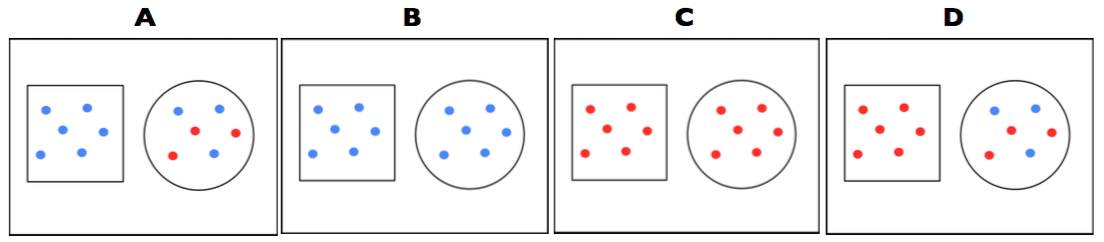
\includegraphics[width = \textwidth]{pics/Augurzky_stimuli.png}
\end{center}

\end{frame}

\begin{frame}{computational-level rational processing}

\textcolor{blue}{general assumptions}

\begin{itemize}
\tightlist
\item
  listener expects speaker to make a pragmatically felicitous utterance
\item
  listener does not give up on speaker rationality on the way (charity,
  forward induction, \ldots{})
\end{itemize}

\textcolor{blue}{experimental microcosmos assumption}

\begin{itemize}
\tightlist
\item
  possible meanings \(\States\): pairs of contexts (\(A\) - \(D\)) and
  speaker-intended shape
\item
  possible messages \(\Messgs\): ``All/some dots are blue/red that are
  in the square/circle.''
\end{itemize}

\textcolor{blue}{specific assumptions}

\begin{itemize}
\tightlist
\item
  listener knows context, but not shape
\item
  speaker chooses description for context and shape
\end{itemize}

\end{frame}

\begin{frame}{next-word expectations vs.~N400}

\begin{itemize}
\tightlist
\item
  incremental RSA predicts \(P_L(w_{i+1} \mid w_{1,\dots,i}, c)\)
\item
  correlating predicted next-word expectations grand-average early N400
  (300-400ms):

  \begin{itemize}
  \tightlist
  \item
    \(r= 0.44\), \(p < 0.01\) in total
  \item
    \(r = 0.81\), \(p < 0.001\) after exclusion of unexpected
    continuations
  \end{itemize}
\end{itemize}

\begin{center}
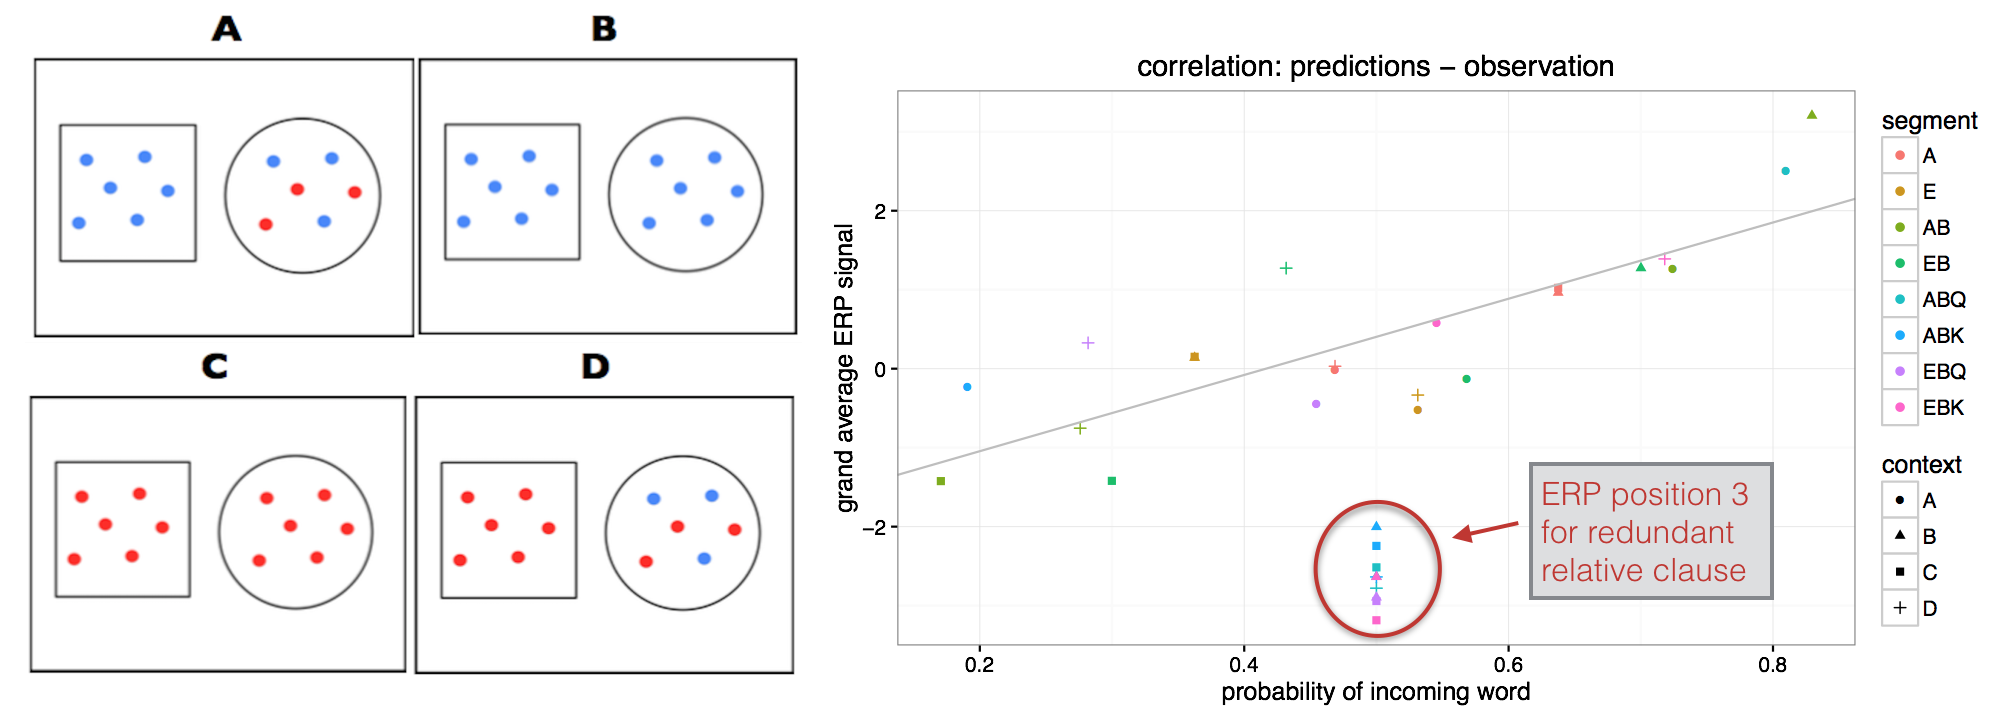
\includegraphics[width = \textwidth]{pics/combined_plots.png}
\end{center}

\end{frame}

\end{document}
